\documentclass{svproc}

% \IEEEoverridecommandlockouts
% \overrideIEEEmargins

\usepackage{amsmath,amssymb,amsfonts}
\usepackage{algorithm}
\usepackage{algorithmic}
\usepackage{cite}
\usepackage{float}
\usepackage{hyperref}
\usepackage{graphicx}
\usepackage{siunitx}
\usepackage{subcaption}
\usepackage{xcolor}

\title{RRT$^\star$ Motion Planning with Control Barrier Function Safety Derived from Poisson Fields}

\author{Maciej Różewicz
    \thanks{Email: rozewicz.maciej@gmail.com}
}

\begin{document}

\mainmatter              % start of a~contribution
%
\title{RRT$^\star$ Motion Planning with Control Barrier Function Safety Derived from Poisson Fields}
%
\titlerunning{RRT$^\star$ Motion Planning with CBF and Poisson Fields}  % abbreviated title (for running head)
%                                     also used for the TOC unless
%                                     \toctitle is used
%
\author{Maciej Różewicz}
%
\authorrunning{Różewicz} % abbreviated author list (for running head)
%
%%%% list of authors for the TOC (use if author list has to be modified)
% \tocauthor{Ivar Ekeland, Roger Temam, Jeffrey Dean, David Grove,
% Craig Chambers, Kim B. Bruce, and Elisa Bertino}
%
\institute{
AGH University of Science and Technology, Kraków, Poland\\
% Aptiv Services Poland\\
\email{mrozewicz@agh.edu.pl}
}

\maketitle              % typeset the title of the contribution
%%%%%%%%%%%%%%%%%%%%%%%%%%%%%%%%%%%%%%%%%%%%%%%%%%%%%%%%%%%%%%%%%%%%%%%%%%%%%%%%%%%%%%%%%
\begin{abstract}
This paper proposes a~novel framework for safe motion planning that integrates
Control Barrier Function (CBF) safety constraints with the Rapidly-Exploring
Random Tree Star (RRT$^\star$) algorithm. The CBF is derived directly from the solution
of a~Poisson equation defined over the free workspace, referred to as
a~\emph{Poisson Safety Function (PSF)}. The PSF encodes obstacle boundaries
and safety gradients in a~smooth, differentiable field that naturally satisfies
Laplace-type spatial regularity. The proposed method, termed
\emph{Safe-CBF-RRT$^\star$}, uses the PSF and its spatial derivatives to enforce
pCBF-based safety conditions along sampled edges during tree expansion. Unlike
pure safety-filter approaches such as FaSTrack, our method actively generates an
inherently safe path while maintaining computational tractability.
Simulation results demonstrate that the method enhances safety and convergence
properties compared to standard RRT$^\star$.
\end{abstract}

%%%%%%%%%%%%%%%%%%%%%%%%%%%%%%%%%%%%%%%%%%%%%%%%%%%%%%%%%%%%%%%%%%%%%%%%%%%%%%%%%%%%%%%%%
\section{Introduction}
In modern robotics applications, ensuring safe navigation in complex
environments is one of the major challenges. This is particularly critical in
scenarios involving human-robot interaction, autonomous vehicles, and
unstructured terrains. Traditional motion planning algorithms often focus on
finding feasible paths without formal guarantees of safety. To achieve such
provable safety, Control Barrier Functions (CBFs) have emerged as a~powerful
tool for enforcing safety constraints in control systems in last years \cite{8796030}. 

In parallel, methods like \textbf{FaSTrack} \cite{Chen_2021} have
provided formal guarantees for \textit{safe trajectory tracking} by defining
a~Safe-to-Track Set ($\mathcal{S}$), leveraging techniques from optimal control
and differential games. However, such methods are primarily safety filters for
the \textit{execution} phase and \textit{do not inherently provide an efficient planner} to
\textit{generate} the safe reference trajectory itself, often suffering from high
computational cost in high-dimensional state spaces.

Sampling-based motion planners such as RRT or RRT$^\star$ are widely used for complex
robotic systems due to their scalability and ability to handle nonconvex
constraints \cite{LaValle1998RapidlyexploringRT},
\cite{karaman2011samplingbasedalgorithmsoptimalmotion}.
However, they rely primarily on geometric collision checking,
offering no formal guarantees of safety. For this reason, integrating CBFs into
sampling-based planners seems to be a~promising direction to enhance safety while
retaining the benefits of sampling-based methods.

A~critical challenge in using CBFs for planning is the construction of
a~suitable safety function $h(x)$, which must be continuously differentiable
and satisfy certain regularity conditions. Analytical definitions of $h(x)$
exist for simple geometries, and lately there have been attempts to get CBF as
solution of Poisson equation \cite{bahati2025dynamicsafetycomplexenvironments},
\cite{BahatiSafeSS}.
This approach will be used in this paper to generate a~Poisson Safety Function
(PSF) that encodes obstacle boundaries and provides smooth safety gradients.
Such definition of $h(x)$ is particularly advantageous for complex environments where
analytical forms are not feasible. Moreover, it seems to be naturally compatible with
the RRT or RRT$^\star$ framework.
\textbf{Contributions:}
In this the \emph{Safe-CBF-RRT$^\star$} framework, the following contributions are made:
\begin{itemize}
    \item integration of the PSF into a~modified RRT$^\star$ algorithm,
    \item a~computationally efficient alternative to tracking-based safety
    methods
    like FaSTrack for generating inherently safe reference trajectories,
    \item simulation results showing improved safety margins and convergence.
\end{itemize}

%%%%%%%%%%%%%%%%%%%%%%%%%%%%%%%%%%%%%%%%%%%%%%%%%%%%%%%%%%%%%%%%%%%%%%%%%%%%%%%%%%%%%%%%%
\section{Related Work}
Sampling-based methods such as RRT and RRT$^\star$ \cite{karaman2011samplingbasedalgorithmsoptimalmotion} have
become standard in high-dimensional motion planning. Extensions incorporating
optimality, dynamics, and risk awareness exist but often lack formal safety guarantees.

Potential field and PDE-based navigation \cite{s22093295} have long
been studied for path planning. Harmonic potential fields, governed by Laplace's
equation, ensure smoothness and avoid local minima, yet they do not directly
provide a~safety margin measurable in the CBF framework.

Control Barrier Functions \cite{8796030,garg2023advancestheorycontrolbarrier} ensure set
invariance in control systems but require a~known differentiable safety
function. Existing methods often define $h(x)$ as analytic distances to
obstacles, which may be nondifferentiable in complex maps. Our approach
bridges this gap by generating $h(x)$ through a~Poisson PDE that respects
boundary geometry.

%========================================================================================
\subsection{Integration of CBFs in Sampling-based Planning}
The integration of Control Barrier Functions with sampling-based planners often
falls into two main categories: those focusing on \textit{control synthesis} and those
focusing on \textit{path filtering}.

\subsubsection{Dynamic and Robust CBF-RRT$^\star$ (Control Synthesis)}
    More advanced methods
    directly incorporate the system's dynamics into the planning process. For example,
    the Robust CBF-RRT$^\star$ approach \cite{Yang_2019} uses CBF conditions, often solved
    via Quadratic Programming (QP), at each time step along a~sampled edge to
    find a~dynamically safe control input $u$. This approach guarantees safety
    for kinodynamic systems and can be extended to Robust CBF (RCBF) to
    handle bounded uncertainties \cite{Yang_2019}. Similarly, methods like
    LQR-CBF-RRT$^\star$ aim for optimality by integrating the Linear Quadratic
    Regulator (LQR) with CBF constraints, sometimes simplifying the process by
    avoiding the continuous QP solving \cite{yang2023lqrcbfrrtsafeoptimalmotion}. While powerful,
    these methods incur a~high online computational cost due to the repeated
    synthesis of safe control (e.g., solving QPs or LQR) during tree expansion.

\subsubsection{Geometric CBF-RRT$^\star$ (Path Filtering)}
    In contrast,
    our method, \emph{Safe-CBF-RRT$^\star$}, uses a~computationally lighter
    approach. It employs a~simplified, discrete CBF condition applied to the
    path segment geometry rather than synthesizing a~dynamic control trajectory.
    This shifts the focus from finding an optimally safe control to generating an
    inherently safe reference path with minimal online computational overhead.

\textbf{Contrast with Tracking-Based Safety Methods (FaSTrack):} Another
influential paradigm for provable safety is the \textit{FaSTrack} framework
\cite{Chen_2021}, which uses level-set methods and
Hamilton-Jacobi-Isaacs (HJI) equations to compute the aforementioned
Safe-to-Track Set ($\mathcal{S}$). While FaSTrack offers strong, worst-case
guarantees against bounded disturbances and execution error,
\textbf{it decouples planning from safety assurance}. The path must first be
planned (e.g., via RRT$^\star$), and then the safe-to-track set is checked for
feasibility, often leading to computationally demanding solutions for
high-dimensional systems. In contrast, \textit{Safe-CBF-RRT$^\star$} integrates the
safety constraint derived from the smooth Poisson field directly into the
sampling and rewiring steps. This allows the planner to efficiently
\textit{generate inherently safe paths}, avoiding the need for expensive
high-dimensional HJI solutions characteristic of FaSTrack-type approaches.

%%%%%%%%%%%%%%%%%%%%%%%%%%%%%%%%%%%%%%%%%%%%%%%%%%%%%%%%%%%%%%%%%%%%%%%%%%%%%%%%%%%%%%%%%
\section{Preliminaries}
%========================================================================================
\subsection{RRT$^\star$ Algorithm}
The RRT$^\star$ algorithm is an incremental, sampling-based motion planner that
asymptotically converges to the optimal feasible path. At each iteration, a~random sample 
$x_{rand}$ is drawn from the state space, and the tree is extended toward this
sample from its nearest node $x_{near}$.
Unlike RRT, RRT$^\star$ performs two additional operations that guarantee asymptotic
optimality. First, it selects a~parent for the new node $x_{new}$ by choosing,
among all nodes within a~ball of radius $r_{n}$, the one that minimizes the
cost-to-come plus the local connection cost. Second, it "rewires" the tree by
checking whether any neighbor can reduce its cost by adopting $x_{new}$ as a~new
parent. As the number of samples $n$ grows, the radius  
$r_{n} = \gamma(\frac{\log{n}}{n})^{\frac{1}{d}}$ shrinks, ensuring both
probabilistic completeness and convergence to the optimal path cost.
This makes RRT$^\star$ suitable for high-dimensional motion planning problems where
exact optimal planning is computationally intractable
\cite{karaman2010incrementalsamplingbasedalgorithmsoptimal},
\cite{karaman2011samplingbasedalgorithmsoptimalmotion}.
Algorithm is summarized in Algorithm~\ref{alg:rrtstar}.
\begin{algorithm}[t]
\caption{Classical RRT$^\star$ algorithm}
\label{alg:rrtstar}
\begin{algorithmic}[1]
\REQUIRE State space $\mathcal{X}$, free space $\mathcal{X}_{\mathrm{free}} \subseteq \mathcal{X}$, 
initial state $x_{\mathrm{init}}$, number of iterations $N$
\STATE $T \gets (\{x_{\mathrm{init}}\}, \emptyset)$
\FOR{$n = 1$ \textbf{to} $N$}
    \STATE $x_{\mathrm{rand}} \sim \mathrm{Unif}(\mathcal{X}_{\mathrm{free}})$
    \STATE $x_{\mathrm{near}} \gets \mathrm{Nearest}(T, x_{\mathrm{rand}})$
    \STATE $x_{\mathrm{new}} \gets \mathrm{Steer}(x_{\mathrm{near}}, x_{\mathrm{rand}})$
    \IF{$\mathrm{CollisionFree}(x_{\mathrm{near}}, x_{\mathrm{new}})$}
        \STATE $\mathcal{N} \gets \mathrm{Neighbors}(T, x_{\mathrm{new}}, r_n)$
        \STATE $x_{\mathrm{parent}} \gets \arg\min\limits_{x \in \mathcal{N}} 
            \left( c(x) + \mathrm{Cost}(x, x_{\mathrm{new}}) \right)$
        \STATE $T.\mathrm{AddNode}(x_{\mathrm{new}})$
        \STATE $T.\mathrm{AddEdge}(x_{\mathrm{parent}}, x_{\mathrm{new}})$
        \FORALL{$x \in \mathcal{N}$}
            \IF{$c(x_{\mathrm{new}}) + \mathrm{Cost}(x_{\mathrm{new}}, x) < c(x)$}
                \STATE $T.\mathrm{Rewire}(x, x_{\mathrm{new}})$
            \ENDIF
        \ENDFOR
    \ENDIF
\ENDFOR
\STATE \RETURN $T$
\end{algorithmic}
\end{algorithm}

%========================================================================================
\subsection{Control Barrier Functions}
Control Barrier Functions (CBFs) provide a~formalism for ensuring safety in
control systems by enforcing forward invariance of a~safe set. Given a~dynamical
system
$
    \dot{x} = f(x) + g(x)u,
$
where $x\in\mathbb{R}^n$ is the state, $u\in\mathbb{R}^m$ is the control input, and
$f,g$ are locally Lipschitz continuous functions, a~set
$
    \mathcal{C} = \{x\in\mathbb{R}^n : h(x) \ge 0\}
$
is defined as \emph{safe} if there exists a~continuously differentiable function
$h:\mathbb{R}^n \to \mathbb{R}$ such that for all $x\in\mathcal{C}$,
$
    \sup_{u\in U} [L_f h(x) + L_g h(x) u] \ge -\kappa h(x),
$
where $L_f h$ and $L_g h$ are the Lie derivatives of $h$ along $f$ and $g$,
respectively, and $\kappa>0$ is a~tuning parameter - the smaller $\kappa$ is
the more conservative is condition. This condition ensures that the system's
trajectories remain within the safe set $\mathcal{C}$ for all future times.

%========================================================================================
\subsection{Poisson Safety Function Generation}
Let $\Omega \subset \mathbb{R}^2$ denote the workspace with boundary
$\partial\Omega$ and obstacles $\mathcal{O}_i$. We define a~vector
potential field $\mathbf{u} = [u_x,u_y]^T$ solving
\begin{equation}
    \left\lbrace
    \begin{array}{ll}
        \nabla^2 \mathbf{u} = 0 & \text{in } \Omega \\
        \mathbf{u} = c_i (\mathbf{x}-\mathbf{c}_i) & \text{on } \partial \mathcal{O}_i
    \end{array}
    \right\rbrace
    .
\end{equation}
A scalar field $h(x,y)$, termed the \emph{Poisson Safety Function (PSF)},
is then obtained by solving
\begin{equation}
    \left\lbrace
    \begin{array}{ll}
        \nabla^2 h = -\|\nabla \mathbf{u}\| & \text{in } \Omega \\
        h|_{\partial\Omega}=0 & \text{on } \partial \mathcal{O}_i
    \end{array}
    \right\rbrace
    ,
\end{equation}
ensuring $h>0$ in free space. Gradients $\nabla h = [\partial h/\partial
x,\partial h/\partial y]$ are computed using finite differences.
% \subsection{Control Barrier Function Constraint}
% For a~path segment between points $a$ and $b$, sampled along $p(s)=a+s(b-a)$,
% $s\in[0,1]$, the discrete CBF condition is
% \begin{equation}
% \nabla h(p) \cdot (b-a) \ge -\kappa h(p)\|b-a\|,
% \end{equation}
% where $\kappa>0$ controls conservatism. This ensures that motion along
% the edge does not approach unsafe regions too rapidly.

%%%%%%%%%%%%%%%%%%%%%%%%%%%%%%%%%%%%%%%%%%%%%%%%%%%%%%%%%%%%%%%%%%%%%%%%%%%%%%%%%%%%%%%%%
\section{Safe CBF-RRT$^\star$ Algorithm}
%========================================================================================
We introduce several key modifications to the classical RRT$^\star$
algorithm in order to incorporate safety constraints derived from
the Poisson-based Control Barrier Function.
\textbf{The most important changes are:}
\begin{enumerate}
    \item \textbf{Edges are validated using a~CBF condition} computed
    from the Poisson Safety Function (PSF) and its spatial gradients.
    \item \textbf{A constant nominal traversal speed is assumed} when
    moving along each candidate edge. This assumption is important: 
    slower motion leads to larger feasible sets under the CBF condition,
    meaning that \emph{even narrow passages may be safe at lower velocities},
    while the same passages are considered unsafe at higher speeds.
    \item \textbf{Edges violating the CBF constraint are rejected},
    preventing unsafe tree expansion even if the geometric collision
    check passes.
    \item \textbf{A safety-weighted cost} is introduced to prefer paths
    that stay in regions with higher PSF values (more safety margin).
\end{enumerate}
Together, these changes turn the sampling process itself into
a~safety-aware procedure, rather than merely filtering an already planned path.

%========================================================================================
\subsection{Ensuring Safety with Poisson CBFs}
The Poisson Safety Function $h(x)$ and its spatial derivatives provide
a~smooth, differentiable representation of obstacle boundaries and safety
gradients. In Safe CBF-RRT$^\star$, these quantities are used in three ways:
\begin{itemize}
    \item \textbf{Discrete CBF validation of each candidate edge.}
    For a~short edge between nodes $a$ and $b$, we assume motion with constant velocity $\dot{x}=v(b-a)/|b-a|$.
    The CBF condition ---,
    sampled at multiple points $p$ along the edge, determines whether traversal is safe.
    This directly links feasibility to assumed speed.
    \item \textbf{Safety-aware cost weighting.}
    Each edge is assigned a~cost depending on both its length and average safety margin $\bar h$.
    \item \textbf{Optional control-feasibility check.}
    For edges that satisfy discrete CBF conditions, PSF gradients can be used to verify whether a~continuous control input exists to maintain safety along the smooth trajectory.
\end{itemize}

%========================================================================================
\subsection{Trajectory Cost with Safety Weighting}
To encourage the planner to use safer portions of the workspace, Safe
CBF-RRT$^\star$ modifies the classical RRT$^\star$ cost function as:
\begin{equation}
J(a,b)=cL + (1-c)\frac{1}{\bar{h}},
\end{equation}
where $L=|b-a|$ is the geometric length, and $\bar{h}$ is the average PSF value along the edge.
Parameter $c\in[0,1]$ determines the trade-off between path efficiency and safety.

%========================================================================================
\subsection{Summary of Safe-CBF-RRT$^\star$}
The overall algorithm follows the standard RRT$^\star$ structure
but rejects edges that fail the CBF feasibility condition
(dependent on assumed traversal speed).
This results in a~tree that grows preferentially through regions
of high safety margin while still preserving the asymptotic optimality
guarantees of RRT$^\star$ for the modified cost.

% A pseudocode outline of the method is shown in Algorithm~\ref{alg:cbfrrt}.
% Safe CBF-RRT$^\star$ integrates the PSF-based CBF constraint into the RRT$^\star$
% framework to ensure safety during tree expansion. The PSF $h(x)$ and its
% derivatives are used in following ways:
% \begin{itemize}
%     \item $h(x)$, $\frac{\partial h(x)}{\partial x}$, $\frac{\partial
%     h(x)}{\partial y}$ are used to fast check if sampled edge is CBF-safe -
%     assume simple constant velocity model along edge,
%     \item $h(x)$ is used to weight path costs - the higher the average $h(x)$
%     along the edge, the safer the edge is considered,
%     \item if simple traversing along the edge is safe then $h(x)$, $\frac{\partial h(x)}{\partial x}$, $\frac{\partial
%     h(x)}{\partial y}$ are used to check if control inputs can be found to
%     keep the system safe with smooth trajectory.
% \end{itemize}

% %========================================================================================
% \subsection{Trajectory cost with safety weighting}
% Safe CBF-RRT$^\star$ extends RRT$^\star$ by filtering edges through CBF validation and
% weighting path costs by safety:
% \begin{align}
% J(a,b) = c L + (1-c)\frac{1}{\bar{h}},
% \end{align}
% where $L=\|b-a\|$, $\bar{h}$ is mean $h$ along the edge, and $c\in[0,1]$
% balances length and safety.

% %========================================================================================
% \subsection{Summary of Safe-CBF-RRT$^\star$}
% The planner iteratively samples, extends, and rewires as in RRT$^\star$, rejecting
% edges that violate the CBF condition. a~pseudocode outline is shown in
% Algorithm~\ref{alg:cbfrrt}.

% \begin{algorithm}[h]
% \caption{Safe-CBF-RRT$^\star$}
% \label{alg:cbfrrt}
% \begin{algorithmic}[1]
% \STATE Initialize tree with $x_{start}$
% \FOR{$k=1:N_{iter}$}
%   \STATE Sample $x_{rand}$
%   \STATE $x_{near} \leftarrow$ Nearest$(x_{rand})$
%   \STATE $x_{new} \leftarrow$ Steer$(x_{near}, x_{rand})$
%   \IF{CollisionFree($x_{near},x_{new}$) and CBFSafe($x_{near},x_{new}$)}
%     \STATE AddNode($x_{new}$); RewireNeighborhood($x_{new}$)
%   \ENDIF
%   \IF{$x_{new}$ near $x_{goal}$}
%     \STATE Connect and return path
%   \ENDIF
% \ENDFOR
% \end{algorithmic}
% \end{algorithm}

%%%%%%%%%%%%%%%%%%%%%%%%%%%%%%%%%%%%%%%%%%%%%%%%%%%%%%%%%%%%%%%%%%%%%%%%%%%%%%%%%%%%%%%%%
\section{Results}
This section presents simulation results comparing Safe-CBF-RRT$^\star$ against standard
RRT$^\star$ in a~2D environment with randomly located obstacles. It provides
diversity of paths, safety margins, and path lengths.

%========================================================================================
\subsection{Simulation Setup}
The workspace was a~square randomly located obstacles. The grid resolution was
$100\times100$. Parameters used were $\text{stepSize}=2$, $\kappa=20$, and
$N_{iter}=2000$.

There were three scenarios with varying obstacle densities and configurations:
\begin{itemize}
    \item \textbf{Scenario I:} Moderately spaced obstacles with few wide corridors.
    \item \textbf{Scenario II:} Tightly packed obstacles with narrow passages
    and one wide corridor.
    \item \textbf{Scenario III:} Few bigger obstacles with one good, wide corridor.
\end{itemize}
Each scenario was run 100 times for both algorithms - it means with $c=1$
(length optimized only) and $c = 0$ (safety optimized only), recording path length,
average safety metric $\bar h$, number of iterations, and rejection ratio to
show how many potntially unsafe segmets are rejected from tree. Scenarios with
$c=1$ are run with two velocities: $2 \frac{m}{s}$ and $0.5 \frac{m}{s}$ to show
ability of Safe-CBF-RRT$^\star$ to find safer paths when moving slower.

Additionally for both algorithm calibrations corresponding iterations were run
with same random seed to show how both algorithms behave in exactly same
conditions.

For simulation purposes, a~simple unicycle kinematic model was assumed:
\begin{equation}
    \left\{
    \begin{array}{c}   
        \dot{x} = v \cos(\theta)\\
        \dot{y} = v \sin(\theta)\\
        \dot{\theta} = \omega
    \end{array}
    \right\}
    .
\end{equation}
%========================================================================================
\subsection{Performance}
%++++++++++++++++++++++++++++++++++++++++++++++++++++++++++++++++++++++++++++++++++++++++
\subsubsection{Scenario I}
Scenario I represents an environment with moderately spaced obstacles and
relatively wide free-space corridors. The PSF field
(Fig.~\ref{fig:scenario_i_h}) exhibits smooth gradients and well-defined
safety basins around obstacles, making it a~representative baseline configuration.
% \begin{figure}[H]
% \begin{center}
%     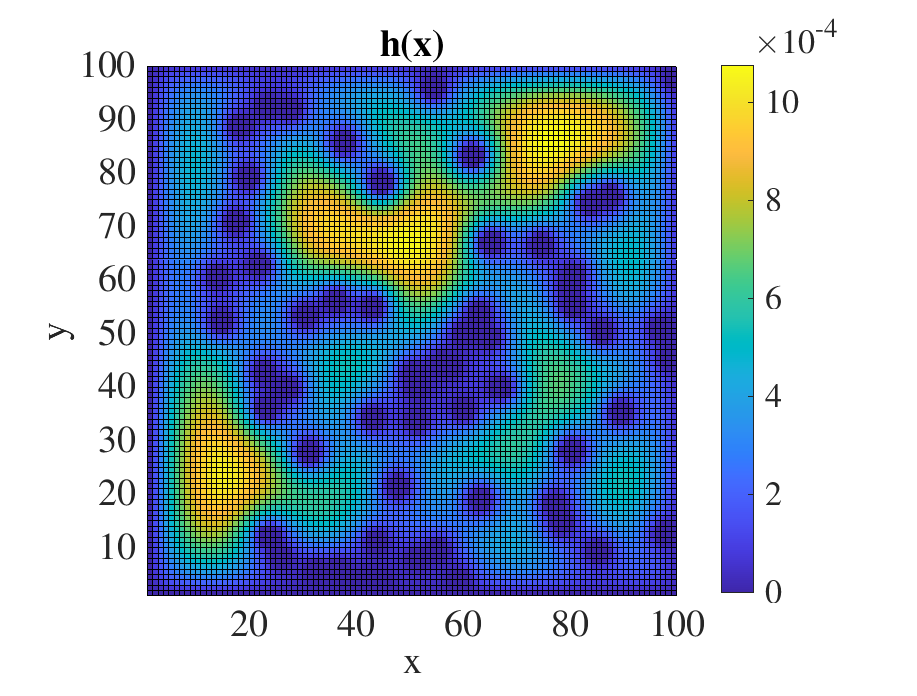
\includegraphics[width=0.5\linewidth]{fig/scenario_i_h}
%     \caption{Control barrier function for Scenario~I.}
%     \label{fig:scenario_i_h}
% \end{center}
% \end{figure}
Standard RRT$^\star$ tends to exploit narrow gaps, often producing shorter but
riskier paths (Fig.~\ref{fig:rrt_without_cbf_scenario_i}). This behavior is
reflected in the low average safety value ($\bar h=0.00057$). In contrast,
Safe-CBF-RRT$^\star$ systematically rejects unsafe edges (48.7\% of samples),
forcing the tree to expand through regions of higher PSF values
(Fig.~\ref{fig:rrt_with_cbf_scenario_i}). As a~result, the mean path length
increases from 118.57 to 147.86, while the mean safety metric improves by ~16\%.
\begin{figure}[h]
\begin{subfigure}{0.5\linewidth}
    \centering
    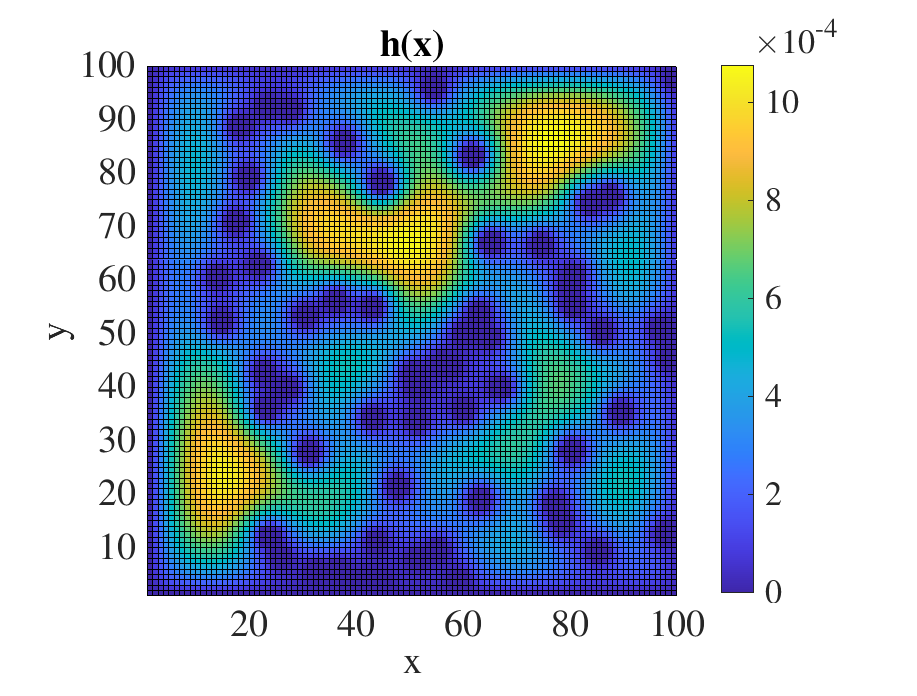
\includegraphics[width=\linewidth]{fig/scenario_i_h}
    \caption{}
    \label{fig:scenario_i_h}
\end{subfigure}
\hfill
\begin{subfigure}{0.5\linewidth}
    \centering
    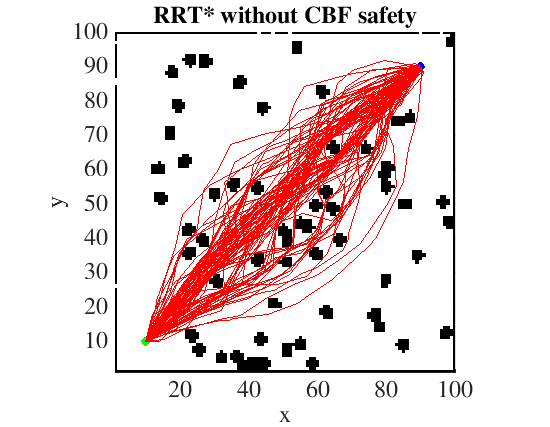
\includegraphics[width=\linewidth]{fig/scenario_i_no_cbf.png}
    \caption{}
    \label{fig:rrt_without_cbf_scenario_i}
\end{subfigure}
\hfill
\begin{subfigure}{0.5\linewidth}
    \centering
    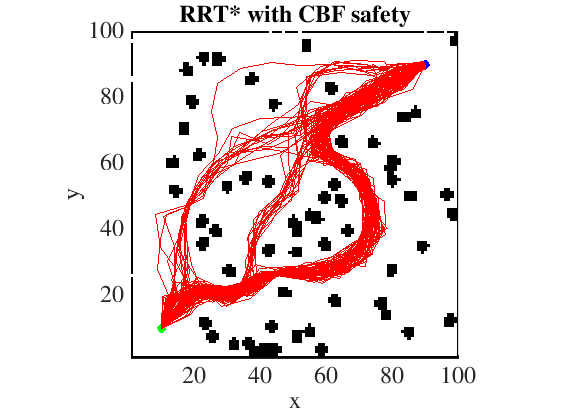
\includegraphics[width=\linewidth]{fig/scenario_i_with_cbf.png}
    \caption{}
    \label{fig:rrt_with_cbf_scenario_i}
\end{subfigure}
\hfill
\begin{subfigure}{0.5\linewidth}
    \centering
    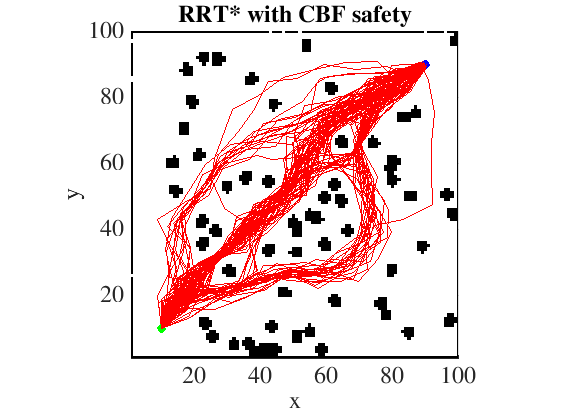
\includegraphics[width=\linewidth]{fig/scenario_i_with_cbf_05ms.png}
    \caption{}
    \label{fig:rrt_with_cbf_scenario_i_05ms}
\end{subfigure}

\caption{Exemple results of 100 different runs for Scenario~I:
(a) Control barrier function,
(b) standard RRT$^\star$,
(c) CBF-RRT$^\star$ for $2 \frac{m}{s}$ target speed,
(d) CBF-RRT$^\star$ for $0.5 \frac{m}{s}$ target speed.}
\label{fig:three_images}
\end{figure}
% \begin{figure}[H]
% \begin{center}
%     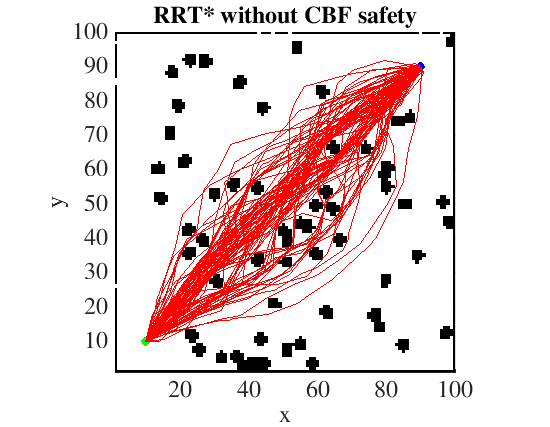
\includegraphics[width=1.0\linewidth]{fig/scenario_i_no_cbf.png}
%     \caption{Exemple results of 100 different runs of standard RRT$^\star$ algorithm for Scenario~I.}
%     \label{fig:rrt_without_cbf_scenario_i}
% \end{center}
% \end{figure}
The higher number of iterations used by CBF-RRT$^\star$ is consistent with
the stronger filtering mechanism, which prioritizes safety over direct
progress toward the goal. Overall, Scenario I demonstrates that the proposed
method effectively increases safety margins even in relatively easy environments.
% \begin{figure}[H]
% \begin{center}
%     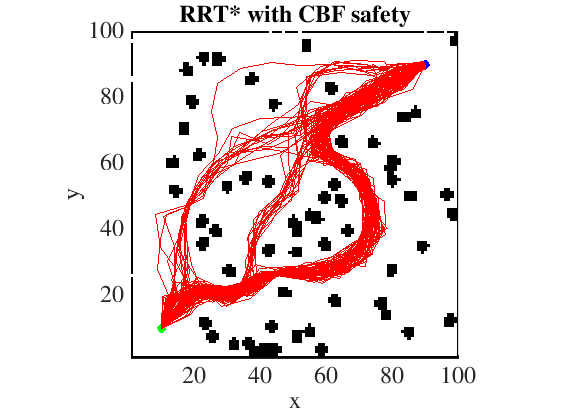
\includegraphics[width=1.0\linewidth]{fig/scenario_i_with_cbf.png}
%     \caption{Exemple results of 100 different runs of CBF-RRT$^\star$
%     algorithm for Scenario~I - for $2 \frac{m}{s}$ target speed.}
%     \label{fig:rrt_with_cbf_scenario_i}
% \end{center}
% \end{figure}
% \begin{figure}[H]
% \begin{center}
%     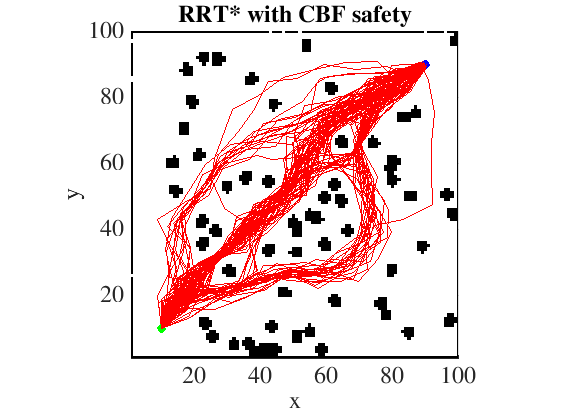
\includegraphics[width=1.0\linewidth]{fig/scenario_i_with_cbf_05ms.png}
%     \caption{Exemple results of 100 different runs of CBF-RRT$^\star$
%     algorithm for Scenario~I - for $0.5\frac{m}{s}$ target speed.}
%     \label{fig:rrt_with_cbf_scenario_i}
% \end{center}
% \end{figure}
For the reduced target speed of $0.5\,\frac{m}{s}$, the impact of the CBF
constraint becomes noticeably weaker. The rejection ratio decreases from 48.7\%
to 27.5\%, and the required number of iterations drops accordingly (372). The
resulting paths remain significantly safer than those generated by standard
RRT$^\star$ ($\bar h=0.00065$), but their geometric length increases only
moderately (128.49), remaining much closer to the baseline RRT$^\star$ solution.
This indicates that at lower target speeds the environment effectively becomes
less restrictive, allowing Safe-CBF-RRT$^\star$ to satisfy the safety
constraints without forcing large detours. Consequently, the planner converges
more efficiently while still benefiting from the PSF-based safety shaping.
\begin{table}[h]
\caption{Performance comparison in Scenario I.}
\begin{center}
\begin{tabular}{|c|c|c|c|c|}
    \hline
    Algorithm       & Length   & $\bar{h}(x)$    & Iterations    &   Rejections\\
    \hline
    RRT$^\star$     & 118.57    & 0.00057   & 333   & 13.6\%   \\
    \hline
    CBF-RRT$^\star\,\left(2\frac{m}{s}\right)$ & 147.86    & 0.00066   & 563   & 48.7\% \\
    \hline
    CBF-RRT$^\star\,\left(0.5\frac{m}{s}\right)$ & 128.49    & 0.00065   & 372   & 27.5\% \\
    \hline
\end{tabular}
\end{center}
\label{tab:performance_scenario_i}
\end{table}

%++++++++++++++++++++++++++++++++++++++++++++++++++++++++++++++++++++++++++++++++++++++++
\subsubsection{Scenario II}
Scenario II introduces significantly tighter passages and higher obstacle density.
The PSF field (Fig.~\ref{fig:scenario_ii_h}) shows steeper gradients and narrow
channels of admissible motion, making safety enforcement more restrictive.
% \begin{figure}[H]
% \begin{center}
%     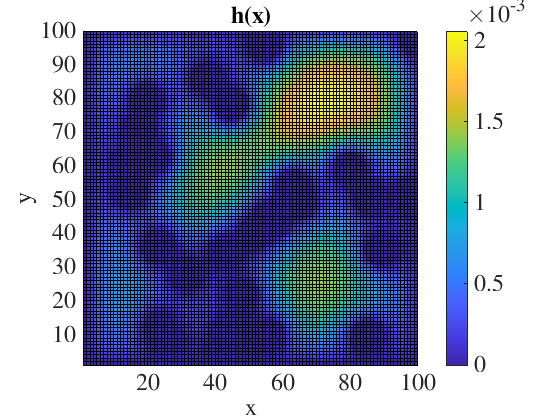
\includegraphics[width=0.5\linewidth]{fig/scenario_ii_h}
%     \caption{Control barrier function for Scenario~II.}
%     \label{fig:scenario_ii_h}
% \end{center}
% \end{figure}
Standard RRT$^\star$ frequently selects unsafe extensions in this environment,
reflected by a~much higher rejection ratio (29.0\%) compared to Scenario I. Its
solutions remain relatively short (119.84), but operate close to obstacles,
maintaining only a~moderate safety average ($\bar h=0.00085$).
\begin{figure}[h]
\begin{subfigure}{0.5\linewidth}
    \centering
    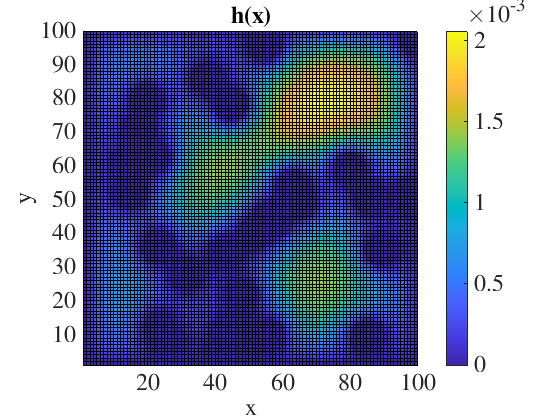
\includegraphics[width=\linewidth]{fig/scenario_ii_h}
    \caption{}
    \label{fig:scenario_ii_h}
\end{subfigure}
\hfill
\begin{subfigure}{0.5\linewidth}
    \centering
    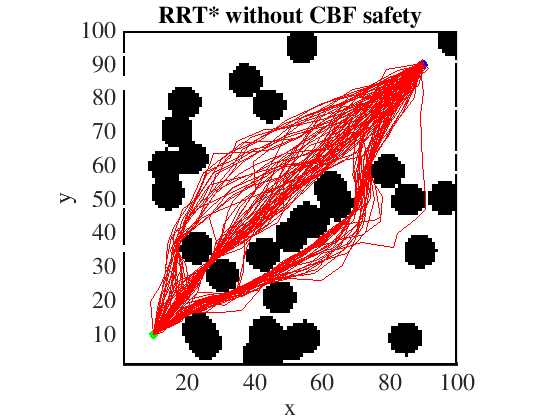
\includegraphics[width=\linewidth]{fig/scenario_ii_no_cbf.png}
    \caption{}
    \label{fig:rrt_without_cbf_scenario_ii}
\end{subfigure}
\hfill
\begin{subfigure}{0.5\linewidth}
    \centering
    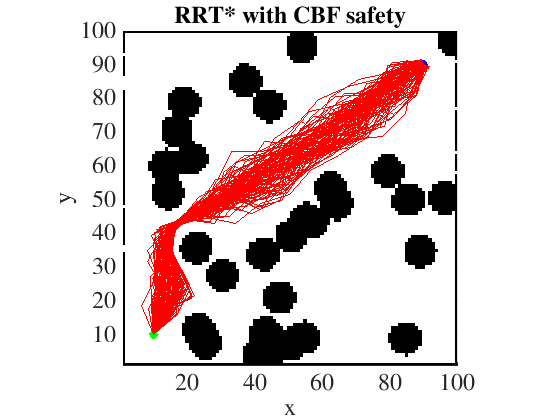
\includegraphics[width=\linewidth]{fig/scenario_ii_with_cbf.png}
    \caption{}
    \label{fig:rrt_with_cbf_scenario_ii}
\end{subfigure}
\hfill
\begin{subfigure}{0.5\linewidth}
    \centering
    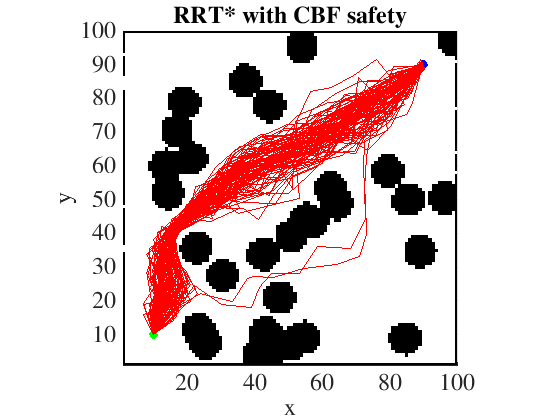
\includegraphics[width=\linewidth]{fig/scenario_ii_with_cbf_05ms.png}
    \caption{}
    \label{fig:rrt_with_cbf_scenario_ii_05ms}
\end{subfigure}
\caption{Exemple results of 100 different runs for Scenario~II:
(a) Control barrier function,
(b) standard RRT$^\star$,
(c) CBF-RRT$^\star$ for $2 \frac{m}{s}$ target speed,
(d) CBF-RRT$^\star$ for $0.5 \frac{m}{s}$ target speed.}
\label{fig:three_images}
\end{figure}
% \begin{figure}[H]
% \begin{center}
%     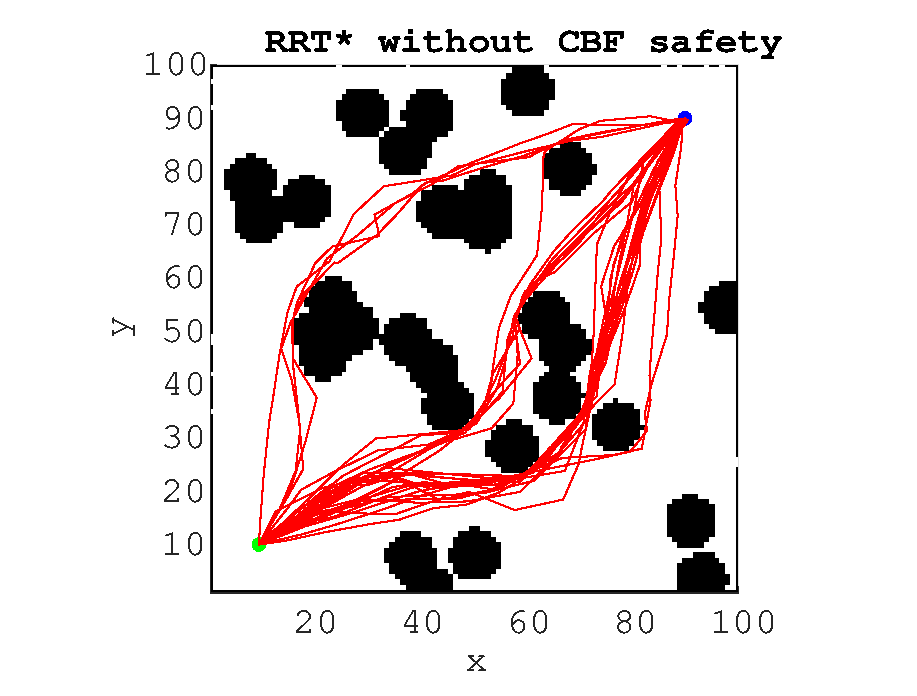
\includegraphics[width=1.0\linewidth]{fig/scenario_ii_no_cbf}
%     \caption{Exemplary 100 different runs of standard RRT$^\star$ algorithm for Scenario~II.}
%     \label{fig:rrt_without_cbf_scenario_ii}
% \end{center}
% \end{figure}
Safe-CBF-RRT$^\star$ must navigate through a~more constrained safety landscape,
leading to an even larger rejection ratio (59.9\%) and correspondingly more
conservative motion. Although the resulting paths are longer (130.95), they
traverse regions with noticeably higher PSF values, improving the average safety
metric by ~29\% relative to standard RRT$^\star$.
% \begin{figure}[H]
% \begin{center}
%     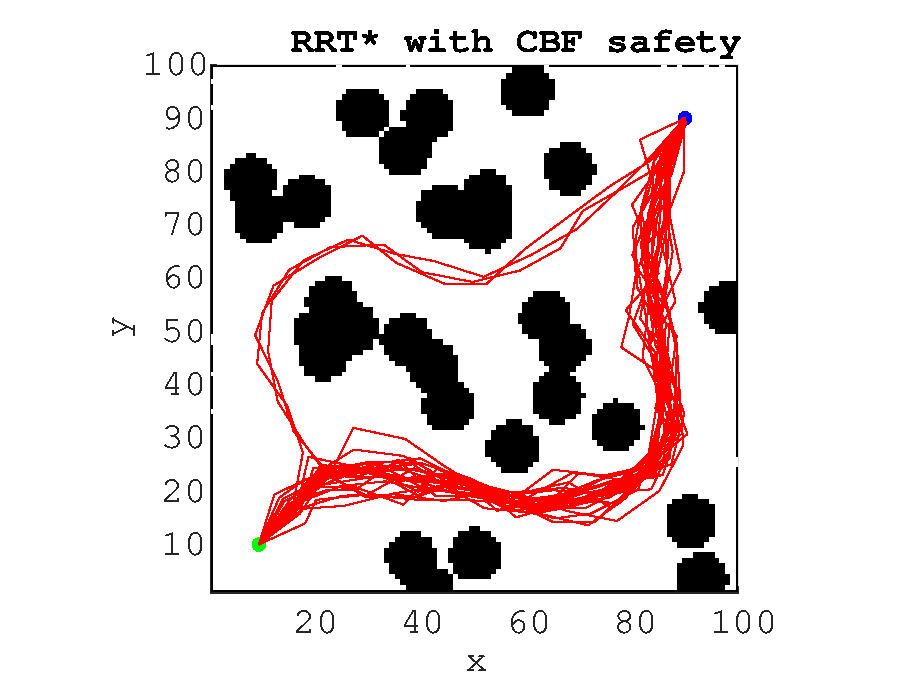
\includegraphics[width=1.0\linewidth]{fig/scenario_ii_with_cbf}
%     \caption{Exemplary 100 different runs of CBF-RRT$^\star$ algorithm for Scenario~II - for $2\frac{m}{s}$ target speed.}
%     \label{fig:rrt_with_cbf_scenario_ii}
% \end{center}
% \end{figure}
Scenario II highlights the ability of the method to maintain safe operation
under geometric constraints that naturally encourage risk-taking behavior
in classical sampling-based planners.
% \begin{figure}[H]
% \begin{center}
%     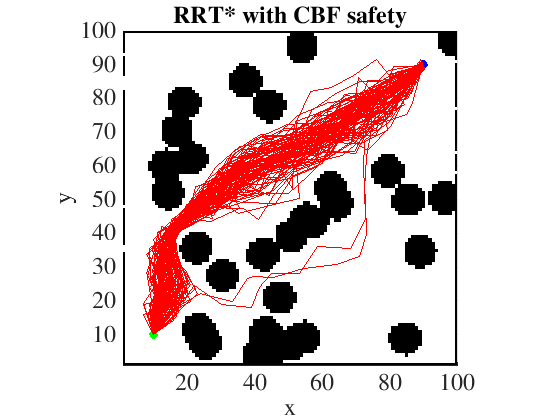
\includegraphics[width=1.0\linewidth]{fig/scenario_ii_with_cbf_05ms.png}
%     \caption{Exemplary 100 different runs of CBF-RRT$^\star$ algorithm for Scenario~II - for $0.5\frac{m}{s}$ target speed.}
%     \label{fig:rrt_with_cbf_scenario_ii}
% \end{center}
% \end{figure}
When the target speed is reduced to $0.5\,\frac{m}{s}$, the CBF filtering
remains strong but becomes considerably less restrictive. The rejection ratio
drops from 59.9\% to 48.5\%, and the number of iterations decreases from 537 to
407, indicating that the planner requires fewer alternative expansions to locate
a safe homotopy class. The resulting trajectories exhibit nearly identical
length (130.80) and safety level ($\bar h=0.00109$) as in the
$2\,\frac{m}{s}$ case. This shows that even in highly constrained environments,
lower forward velocity relaxes the safety constraint sufficiently to reduce
computational effort while preserving the safety benefits of the proposed
method.
\begin{table}[h]
\caption{Performance comparison in Scenario II.}
\begin{center}
\begin{tabular}{|c|c|c|c|c|}
    \hline
    Algorithm       & Length   & $\bar{h}(x)$    & Iterations    &   Rejections\\
    \hline
    RRT$^\star$     & 119.84    & 0.00085   & 345   & 29.0\%   \\
    \hline
    CBF-RRT$^\star\,\left(2\frac{m}{s}\right)$ & 130.95    & 0.00110   & 537   & 59.9\% \\
    \hline
    CBF-RRT$^\star\,\left(0.5\frac{m}{s}\right)$ & 130.80    & 0.00109   & 407   & 48.5\% \\
    \hline
\end{tabular}
\end{center}
\label{tab:performance_scenario_ii}
\end{table}

%++++++++++++++++++++++++++++++++++++++++++++++++++++++++++++++++++++++++++++++++++++++++
\subsubsection{Scenario III}
Scenario III consists primarily of an open environment with a~few concentrated
high-risk areas. The PSF distribution (Fig.~\ref{fig:scenario_iii_h}) features
broad low-gradient regions interspersed with sharp drops near obstacles.
% \begin{figure}[H]
% \begin{center}
%     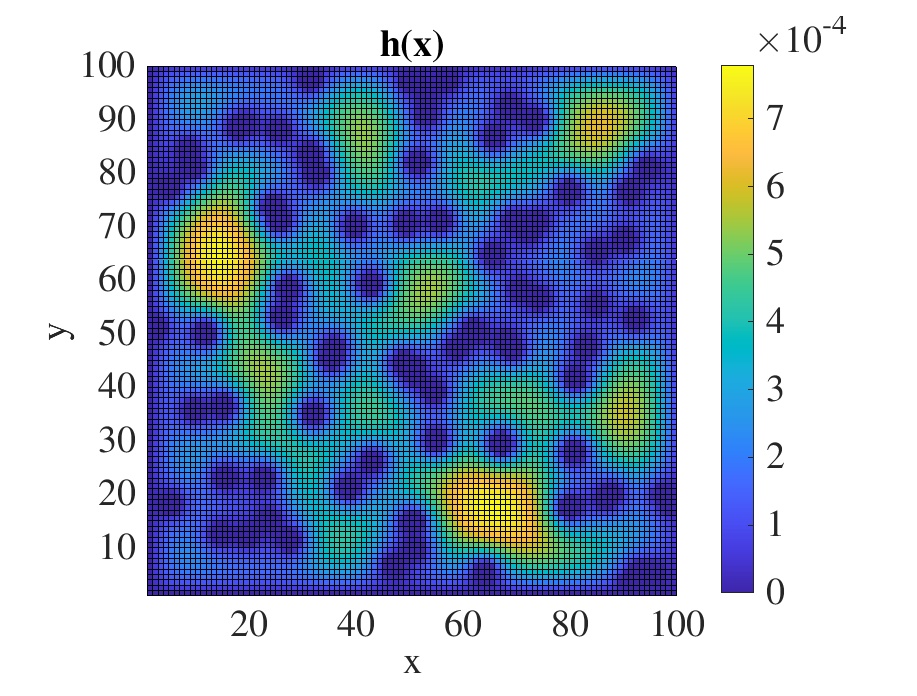
\includegraphics[width=0.5\linewidth]{fig/scenario_iii_h}
%     \caption{Exemplary 100 different runs of standard RRT$^\star$ algorithm.}
%     \label{fig:scenario_iii_h}
% \end{center}
% \end{figure}
In this configuration, standard RRT$^\star$ is able to find relatively direct
paths (122.71), but due to the scattered obstacle layout, it often crosses
regions of low safety potential. This is reflected in the lowest average safety
value among all scenarios ($\bar h=0.00037$).
\begin{figure}[h]
\begin{subfigure}{0.5\linewidth}
    \centering
    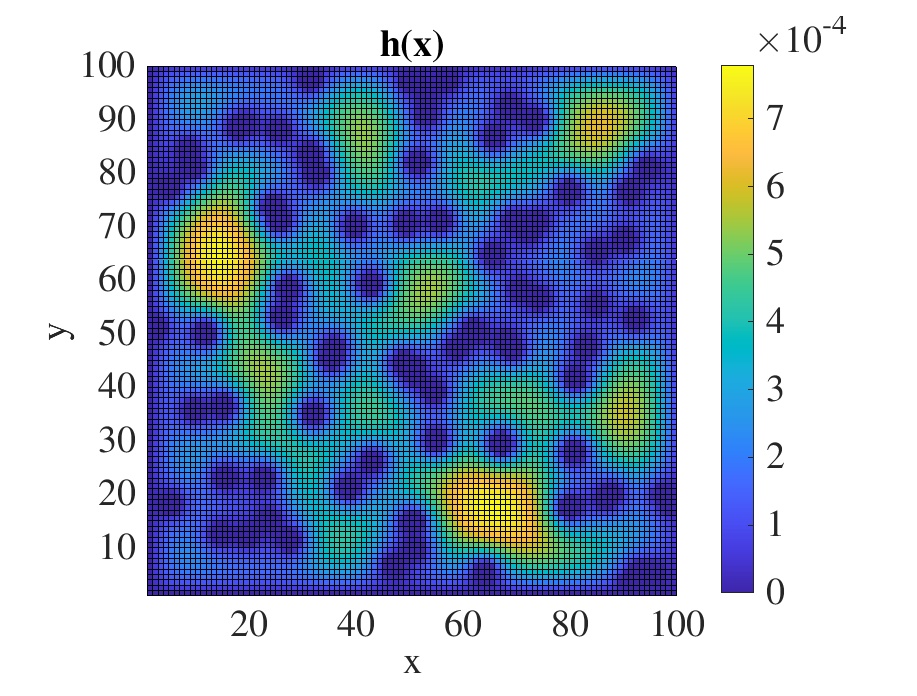
\includegraphics[width=\linewidth]{fig/scenario_iii_h}
    \caption{}
    \label{fig:scenario_iii_h}
\end{subfigure}
\hfill
\begin{subfigure}{0.5\linewidth}
    \centering
    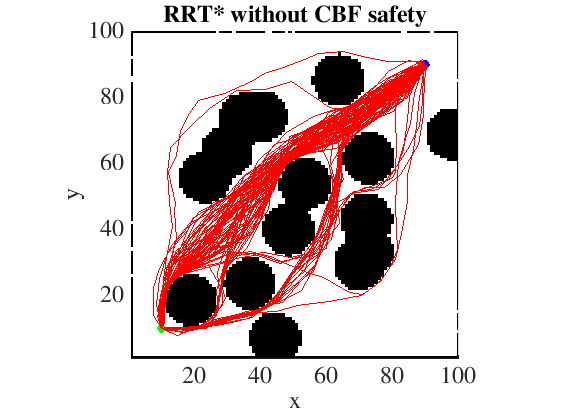
\includegraphics[width=\linewidth]{fig/scenario_iii_no_cbf.png}
    \caption{}
    \label{fig:rrt_without_cbf_scenario_iii}
\end{subfigure}
\hfill
\begin{subfigure}{0.5\linewidth}
    \centering
    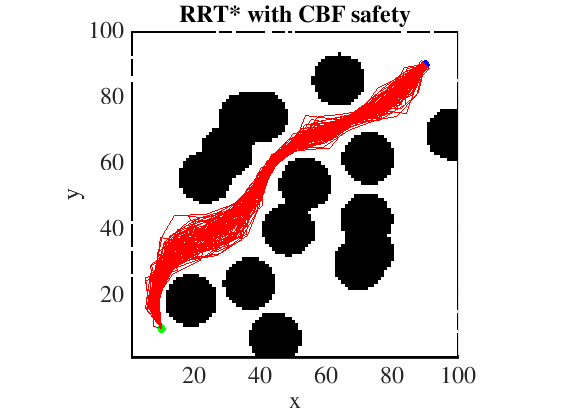
\includegraphics[width=\linewidth]{fig/scenario_iii_with_cbf.png}
    \caption{}
    \label{fig:rrt_with_cbf_scenario_iii}
\end{subfigure}
\hfill
\begin{subfigure}{0.5\linewidth}
    \centering
    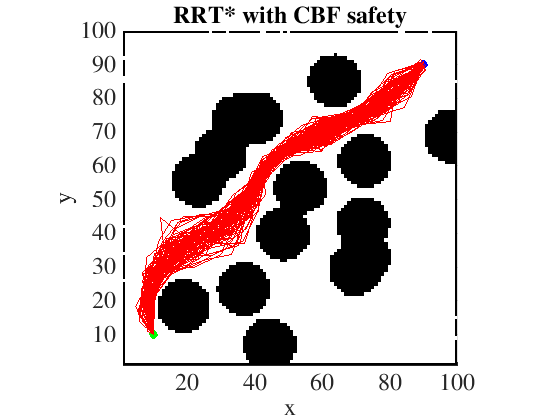
\includegraphics[width=\linewidth]{fig/scenario_iii_with_cbf_05ms.png}
    \caption{}
    \label{fig:rrt_with_cbf_scenario_iii_05ms}
\end{subfigure}
\caption{Exemple results of 100 different runs for Scenario~III:
(a) Control barrier function,
(b) standard RRT$^\star$,
(c) CBF-RRT$^\star$ for $2 \frac{m}{s}$ target speed,
(d) CBF-RRT$^\star$ for $0.5 \frac{m}{s}$ target speed.}
\label{fig:three_images}
\end{figure}
% \begin{figure}[H]
% \begin{center}
%     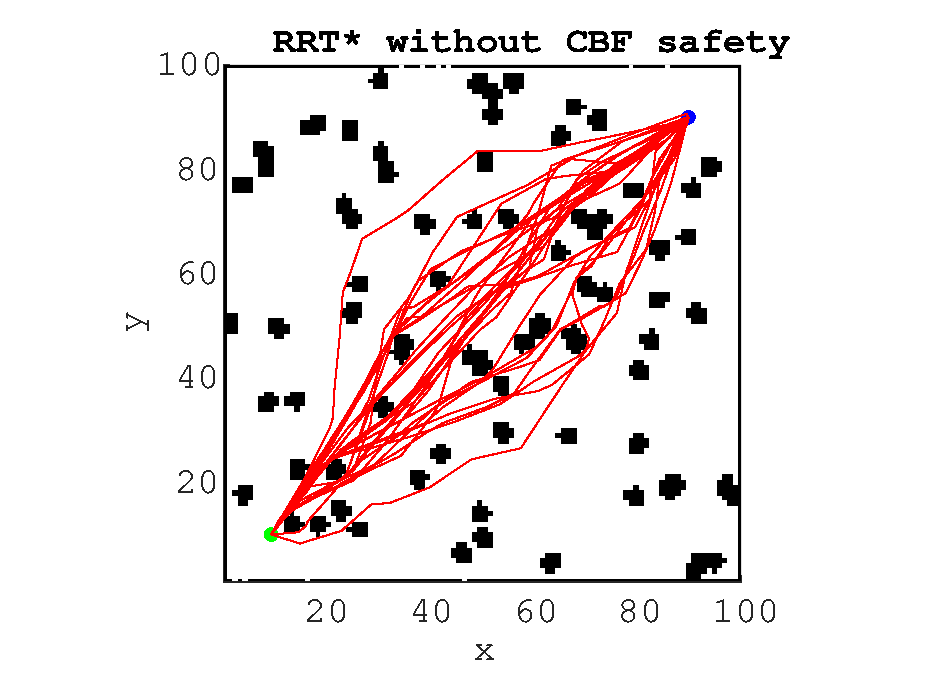
\includegraphics[width=1.0\linewidth]{fig/scenario_iii_no_cbf}
%     \caption{Exemplary 100 different runs of standard RRT$^\star$ algorithm for Scenario~III.}
%     \label{fig:rrt_without_cbf_scenario_iii}
% \end{center}
% \end{figure}
Safe-CBF-RRT$^\star$ improves the safety metric to $\bar h=0.00048$ by rejecting
58.4\% of unsafe expansions and steering the tree around low-PSF zones
(Fig.~\ref{fig:rrt_with_cbf_scenario_iii}). Interestingly, the number of
iterations is slightly lower than for standard RRT$^\star$, indicating that
large open areas reduce the need for rewiring and costly exploration. Despite
the safety constraints, the method only marginally increases the path length
(from 122.71 to 126.32), demonstrating that when safe alternatives are abundant,
the penalty for enforcing CBF constraints becomes minimal.
% \begin{figure}[H]
% \begin{center}
%     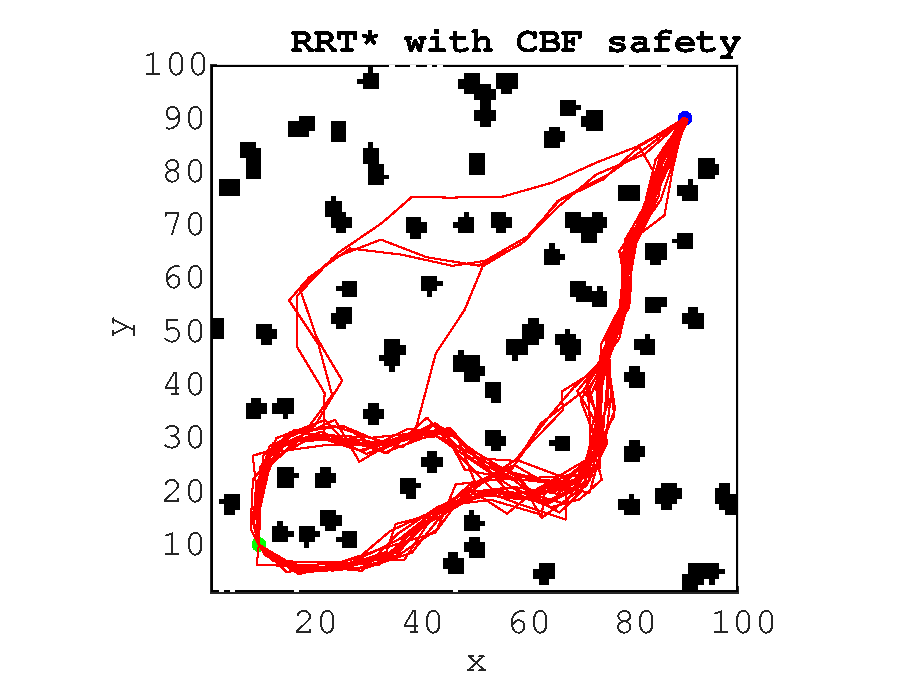
\includegraphics[width=1.0\linewidth]{fig/scenario_iii_with_cbf}
%     \caption{Exemplary 100 different runs of CBF-RRT$^\star$ algorithm for Scenario~III - for $2\frac{m}{s}$ target speed.}
%     \label{fig:rrt_with_cbf_scenario_iii}
% \end{center}
% \end{figure}
Scenario III shows that the proposed planner adapts gracefully to environments
where safe path options are naturally available, avoiding unnecessary
conservatism while still improving safety.
% \begin{figure}[H]
% \begin{center}
%     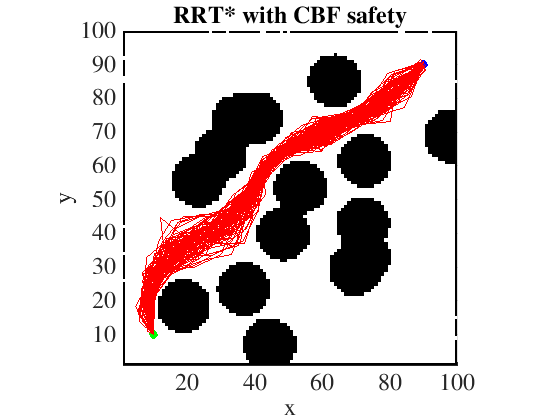
\includegraphics[width=1.0\linewidth]{fig/scenario_iii_with_cbf_05ms.png}
%     \caption{Exemplary 100 different runs of CBF-RRT$^\star$ algorithm for Scenario~III - for $0.5\frac{m}{s}$ target speed.}
%     \label{fig:rrt_with_cbf_scenario_iii}
% \end{center}
% \end{figure}
For the reduced speed of $0.5\,\frac{m}{s}$, the planner benefits from the
abundance of safe alternatives: the rejection ratio decreases from 58.4\% to
48.7\%, and the number of iterations further drops to 362. Despite this, the
safety level remains essentially unchanged ($\bar h=0.00047$), and the resulting
trajectory length (126.51) stays very close to the
$2\,\frac{m}{s}$ variant. This confirms that in open environments the influence
of the CBF constraint diminishes at lower speeds, since safe feasible expansions
are readily available, and the planner does not require significant detours to
maintain conservative operation.
\begin{table}[h]
\caption{Performance comparison in Scenario III.}
\begin{center}
\begin{tabular}{|c|c|c|c|c|}
    \hline
    Algorithm       & Length   & $\bar{h}(x)$    & Iterations    &   Rejections\\
    \hline
    RRT$^\star$     & 122.71    & 0.00037   & 421   & 39.8\%   \\
    \hline
    CBF-RRT$^\star\,\left(2\frac{m}{s}\right)$ & 126.32    & 0.00048   & 389   & 58.4\% \\
    \hline
    CBF-RRT$^\star\,\left(0.5\frac{m}{s}\right)$ & 126.51    & 0.00047   & 362   & 48.7\% \\
    \hline
\end{tabular}
\end{center}
\label{tab:performance_scenario_iii}
\end{table}

\section{Discussion}
Evaluation across three scenarios confirms that integrating PSF-based CBF
constraints significantly biases the planner toward safer regions,
establishing a~clear trade-off between path length and safety margins.

\begin{itemize}
    \item \textbf{Scenario I (Wide Corridors):} Safe-CBF-RRT$^\star$ filtered
    $\sim$50\% of candidate edges. While this led to moderate path elongation,
    it ensured trajectories with consistently higher safety margins ($\bar{h}$)
    than standard RRT$^\star$.
    \item \textbf{Scenario II (Dense Obstacles):} The filtering effect was most
    pronounced here. Standard RRT$^\star$ favored risky, narrow gaps, whereas
    the proposed method pruned these unsafe homotopy classes early, forcing
    exploration of safer, albeit longer, detours and improving $\bar{h}$ by 29\%.
    \item \textbf{Scenario III (Sparse Environment):} In open spaces, both
    planners performed similarly. But, the PSF-weighted cost function
    still biased rewiring toward more robust paths, proving the method maintains
    efficiency without degrading performance in simple environments.
\end{itemize}

\noindent \textbf{Analysis of Behavior:}
\begin{enumerate}
    \item \textbf{Global Influence:} Seed-identical comparisons show the CBF
    constraint reshapes the tree structure from early exploration, rather than
    acting as a~post-filter.
    \item \textbf{Tunability:} Adjusting $c$ allows a~continuous trade-off
    between geometric optimality ($c=1$) and risk minimization ($c=0$),
    adaptable to various safety-critical applications.
    \item \textbf{Efficiency:} Despite higher rejection rates, the algorithm
    maintains stable convergence, ensuring safe trajectories at a~lower
    cost than HJI-based methods.
\end{enumerate}

%%%%%%%%%%%%%%%%%%%%%%%%%%%%%%%%%%%%%%%%%%%%%%%%%%%%%%%%%%%%%%%%%%%%%%%%%%%%%%%%%%%%%%%%%
\section{Conclusion and Future Work}
We presented \emph{Safe-CBF-RRT$^\star$}, a~motion planning framework combining RRT$^\star$
with a~Control Barrier Function derived from a~Poisson Safety Field. The
approach unifies PDE-based potential field generation with formal safety
guarantees \textbf{in a~manner computationally lighter than tracking-based
methods (e.g., FaSTrack)}, while actively shaping the path for safety. Future
work will extend this method to kinodynamic models, uncertain
environments, and real robotic experiments.

%%%%%%%%%%%%%%%%%%%%%%%%%%%%%%%%%%%%%%%%%%%%%%%%%%%%%%%%%%%%%%%%%%%%%%%%%%%%%%%
\bibliographystyle{abbrv}
\bibliography{refs}

\end{document}